\documentclass[a4paper,10pt,twoside,final,spanish]{article}

% Preámbulo - Parte A

\usepackage[utf8]{inputenc} % Soporte para los acentos
\usepackage[T1]{fontenc}

\usepackage[spanish]{babel} % Capítulos, seciones, etc. en español

\usepackage[margin=2cm]{geometry} % Diseño del documento

\usepackage{multicol} % Escribir doble columna

\usepackage{xcolor} % Usar colores
\usepackage{pstricks}

\usepackage{enumerate} % Cambiar etiquetas de numeración
\usepackage[shortlabels]{enumitem} % Manejo adicional de etiquetas de numeración

\usepackage{graphicx} % Manejo de gráficos y figuras

\usepackage{makeidx} % Índice alfabético

% Paquetes adicionales de símbolos matemáticos
\usepackage{amsmath,amssymb,amsfonts,latexsym} 

% \usepackage{pslatex} % Fuente Times
% \usepackage{mathpazo} % Fuente Palatino
% \usepackage{mathptmx} % Fuente Times
% \usepackage{bookman} % Fuente Bookman
\usepackage{newcent} % Fuente New Century Schoolbook
% \usepackage{helvet} % Fuente Helvetica
% \usepackage{palatino} % Fuente Palatino
% \usepackage{pxfonts} % Fuente 
% \usepackage{txfonts} % Fuente
% \usepackage{concrete} % Fuente
% \usepackage{cmbright} % Fuente
% \usepackage{fourier} % Fuente

\usepackage{booktabs} % Opciones adicionales para el entorno tabular
\usepackage{longtable} % Para tablas de más de una página

\usepackage{tikz,tkz-tab} % Creación de gráficos
	\usetikzlibrary{matrix,arrows,positioning,shadows,shadings,
					backgrounds,calc,shapes,tikzmark}
\usepackage{tcolorbox,empheq} % Creación de cajas
	\tcbuselibrary{skins,breakable,listings,theorems}
	
%	\tcbset{opteqC/.style={skin=beamer,colback=red!5!white}}

\usepackage{hyperref}

\usepackage{gensymb} % Grados Celcius

\usepackage{textcomp}

\usepackage[makeroom]{cancel} %Para tachar expresiones matemáticas
\newcommand\Ccancel[2][black]{\renewcommand\CancelColor{\color{#1}}\cancel{#2}}

\usepackage{soul} % para tachar texto
\pagestyle{headings}
% Para encerrar expresiones con círculos
\usepackage{mathtools}% superior to amsmath
\usepackage{siunitx} % para escribir grados minutos segundos
\usepackage{tikz}
\makeatletter
\newcommand\mathcircled[1]{%
  \mathpalette\@mathcircled{#1}%
}
\newcommand\@mathcircled[2]{%
  \tikz[baseline=(math.base)] \node[draw,circle,inner sep=1pt] (math) {$\m@th#1#2$};%
}
\makeatother
%---
\usepackage{fancyhdr} %Para usar encabezados y pies personalizados
	\pagestyle{fancy}
	\fancyhf{}
	\fancyhead[LE,RO]{Mecánica del Continuo}
	\fancyhead[RE,LO]{Ecuaciones Constitutivas}
	\fancyfoot[LE,RO]{\thepage}
	\fancyfoot[RE,LO]{Darién Julián Ramírez}	
	\renewcommand{\footrulewidth}{1pt}
%---
\usepackage{listings} %Para escribir códigos
\lstset{language=XML,
	basicstyle=\footnotesize,
	numbers=left,
 	stepnumber=1,
	numbersep=8pt,
	showspaces=false,               % show spaces adding particular underscores
  	showstringspaces=false,         % underline spaces within strings
  	frame=lines,                   % adds a frame around the code
	tabsize=4,                      
  	captionpos=b,                   % sets the caption-position to bottom
  	breaklines=true,                % sets automatic line breaking
}
%---

% Preámbulo - Parte B

\title{\Huge Mecánica del Continuo \\
			 Trabajo Práctico Nº7  \\
			 Ecuaciones Constitutivas}
\author{Darién Julián Ramírez}
\date{}

% Cuerpo del documento

\begin{document}

\maketitle % Mostrar título

\section*{Ejercicio 1}

Muestre que la \textit{Ley de Hooke}:

\begin{align*}
\sigma_{ij} &= \lambda e_{\alpha\alpha}\delta_{ij}+2\mu e_{ij}
\end{align*}

puede escribirse como

\begin{align*}
e_{xx}=\frac{1}{E}(\sigma_{xx}-\nu(\sigma_{yy}+\sigma_{xx}))
&& e_{xy} &= \frac{1+\nu}{E}\sigma_{xy} \\
e_{yy}=\frac{1}{E}(\sigma_{yy}-\nu(\sigma_{xx}+\sigma_{zz}))
&& e_{yz} &= \frac{1+\nu}{E}\sigma_{yz} \\
e_{zz}=\frac{1}{E}(\sigma_{zz}-\nu(\sigma_{xx}+\sigma_{yy}))
&& e_{zx} &= \frac{1+\nu}{E}\sigma_{zx}
\end{align*}

si $E$ y $\nu$ se relacionan con las contantes de \textit{Lamé} de acuerdo a las siguientes relaciones:

\begin{align*}
\lambda &= \frac{E\nu}{(1+\nu)(1-2\nu)}           &
G=\mu   &= \frac{E}{2(1+\nu)}                     &
E       &= \frac{\mu(3\lambda+2\mu)}{\lambda+\mu} &
\nu     &= \frac{\lambda}{2(\lambda+\mu)}         &
\end{align*}

\dotfill

\begin{quote}

%[opteqC]
\begin{tcolorbox}[colback=gray!10!white,colframe=black!0!white]

Cuando $i\neq j$:

\begin{align*}
\sigma_{xy} &= \lambda e_{\alpha\alpha}\delta_{xy}+2\mu e_{xy} & \delta_{xy} &= 0 \\
&= 2\mu e_{xy} & \mu &= \frac{E}{2(1+\nu)} \\
&= \frac{2E}{2(1+\nu)}e_{xy} & \textit{Simplificando} \\
&= \frac{E}{(1+\nu)}e_{xy} & \textit{Despejando} \\
\frac{(1+\nu)}{E}\sigma_{xy} &= e_{xy}
\end{align*}

\end{tcolorbox}

\begin{tcolorbox}[colback=gray!10!white,colframe=black!0!white]

Paso de expresar la tensión en función de la deformación a expresar la deformación en función de la tensión:

\begin{align*}
\sigma_{ii} &= \lambda e_{\alpha\alpha}\delta_{ii}+2\mu e_{ii}
& e_{\alpha\alpha} &= 3e_{ii} \\
&& \delta_{ii} &= 1 \\
&= 3\lambda e_{ii}+2\mu e_{ii} & \textit{Factor común} \\
&= (3\lambda+2\mu)e_{ii} & \textit{Despejando} \\
\frac{1}{(3\lambda+2\mu)}\sigma_{ii} &= e_{ii} \\
\end{align*}

\end{tcolorbox}

\begin{tcolorbox}[colback=gray!10!white,colframe=black!0!white]

Cuando $i=j$:

\begin{align*}
\sigma_{xx} &= \lambda e_{\alpha\alpha}\delta_{xx}+2\mu e_{xx} 
& e_{\alpha\alpha} &= \frac{1}{(3\lambda+2\mu)}\sigma_{\alpha\alpha} \\
&& \delta_{xx} &= 1 \\
&= \frac{\lambda}{(3\lambda+2\mu)}\sigma_{\alpha\alpha}+2\mu e_{xx}
& \sigma_{\alpha\alpha} &= \sigma_{xx}+\sigma_{yy}+\sigma_{zz} \\
&= \frac{\lambda}{(3\lambda+2\mu)}(\sigma_{xx}+\sigma_{yy}+\sigma_{zz})+2\mu e_{xx}
& \textit{Despejando} \\
e_{xx} &= \frac{1}{2\mu}\left(\sigma_{xx}-\frac{\lambda}{(3\lambda+2\mu)}(\sigma_{xx}+\sigma_{yy}+\sigma_{zz})\right)
& \textit{Factor común} \\
&= \frac{1}{2\mu(3\lambda+2\mu)}\left((3\lambda+2\mu)\sigma_{xx}-\lambda(\sigma_{xx}+\sigma_{yy}+\sigma_{zz})\right) 
& \textit{Distribuyendo} \\
&= \frac{1}{2\mu(3\lambda+2\mu)}\left((3\lambda+2\mu)\sigma_{xx}-\lambda\sigma_{xx}-\lambda(\sigma_{yy}+\sigma_{zz})\right) & \textit{Factor común}\\
&= \frac{1}{2\mu(3\lambda+2\mu)}\left((3\lambda+2\mu-\lambda)\sigma_{xx}-\lambda(\sigma_{yy}+\sigma_{zz})\right) & \textit{Sumando}\\
&= \frac{1}{2\mu(3\lambda+2\mu)}\left(2(\lambda+\mu)\sigma_{xx}-\lambda(\sigma_{yy}+\sigma_{zz})\right) & \textit{Factor común} \\
&= \frac{2(\lambda+\mu)}{2\mu(3\lambda+2\mu)}\left(\sigma_{xx}-\frac{\lambda}{2(\lambda+\mu)}(\sigma_{yy}+\sigma_{zz})\right)
& \nu &= \frac{\lambda}{2(\lambda+\mu)} \\
&= \frac{(\lambda+\mu)}{\mu(3\lambda+2\mu)}\left(\sigma_{xx}-\nu(\sigma_{yy}+\sigma_{zz})\right)
& \frac{1}{E} &= \frac{\lambda+\mu}{\mu(3\lambda+2\mu)} \\
&= \frac{1}{E}\left(\sigma_{xx}-\nu(\sigma_{yy}+\sigma_{zz})\right)
\end{align*}

\end{tcolorbox}

\end{quote}

\section*{Ejercicio 2}

Considere un flujómetro de \textit{Couette} de la figura

\begin{center}
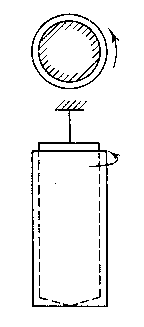
\includegraphics{couette}
\end{center}

Obtenga la distribución de velocidades en el canal, la expresión de la viscosidad del 
fluido, y la relación torque-angular, $T=f(\omega)$. Finalmente, analice cómo cambia  el torque para ensayos realizados con distintos fluidos a la misma velocidad angular. 

\dotfill

\begin{quote}

\begin{align*}
T &= \tau (2\pi rL)r \\
&= 2\pi Lr^{2}\tau & \tau &= \mu\frac{\partial v_{\theta}}{\partial r} \\
&= 2\pi Lr^{2}\mu\frac{\partial v_{\theta}}{\partial r}
\end{align*}

\begin{align*}
v_{\theta}(r=R_{1}) &= 0 \\
v_{\theta}(R_{1}) &= \frac{T}{2\pi L\mu}\left(-\frac{1}{R_{1}}+C\right)=0
& C &= \frac{1}{R_{1}}
\end{align*}

\begin{align*}
\frac{\partial v_{\theta}}{\partial r} &= \frac{T}{2\pi L r^{2}\mu} \\
v_{\theta} &= \int\frac{T}{2\pi L r^{2}\mu}dr
=\frac{T}{2\pi L\mu}\left(-\frac{1}{r}+C\right)
\end{align*}

\begin{align*}
v_{\theta}(r) &= \frac{T}{2\pi L\mu}\left(-\frac{1}{r}+\frac{1}{R_{1}}\right) \\
v_{\theta}(r=R_{2}) &= \omega R_{2}
=\frac{T}{2\pi L\mu}\left(\frac{1}{R_{1}}-\frac{1}{R_{2}}\right) \\
\mu &= \frac{T}{2\pi L\omega R_{2}}\left(\frac{1}{R_{1}}-\frac{1}{R_{2}}\right) \\ \\
T &= \frac{2\pi L\omega R_{2}\mu}{\frac{1}{R_{1}}-\frac{1}{R_{2}}}
\end{align*}

\end{quote}

\section*{Ejercicio 3}

Considere un estado bidimensional de tensiones en una placa delgada en la cual $\sigma_{z}=\tau_{zx}=\tau_{zy}=0$. Las ecuaciones de equilibrio actuando en la placa  con cargas distribuidas de cuerpo $X,Y$ (constantes) son

\begin{align*}
\frac{\partial\sigma_{x}}{\partial x}
+\frac{\partial\tau_{xy}}{\partial y}+X &= 0 \\
\frac{\partial\tau_{xy}}{\partial x}
+\frac{\partial\sigma_{y}}{\partial y}+Y &= 0
\end{align*}
 
Sabemos que estas ecuaciones se satisfacen idénticamente si $\sigma_{x},\sigma_{y},\tau_{xy}$ se derivan de una función arbitraria  $\Phi(x,y)$ en la forma (ver Guía 3): 

\begin{align*}
\sigma_x &= \frac{\partial^{2}\Phi}{\partial y^{2}} \\
\sigma_y &= \frac{\partial^{2}\Phi}{\partial x^{2}} \\
\tau_{xy} &= -\frac{\partial^{2}\Phi}{\partial x \partial y}-Xy-Yx
\end{align*}

\begin{enumerate}[a.]
\item Demostrar que para un material elástico lineal, para el cual se verifica:

\begin{align*}
e_{xx} &= \frac{1}{E}(\sigma_{x}-\nu\sigma_{y}) \\
e_{yy} &= \frac{1}{E}(\sigma_{y}-\nu\sigma_{x}) \\
e_{xy} &= \frac{\tau_{xy}}{G}=\frac{(1+\nu)}{E}\tau_{xy}
\end{align*}

las condiciones de compatibilidad se verifican si y solo si:

\begin{align*}
\nabla^{4}\Phi &= \frac{\partial^{4}\Phi}{\partial x^{4}}
+2\frac{\partial^{4}\Phi}{\partial x^{2} \partial y^{2}}
+\frac{\partial^{4}\Phi}{\partial y^{4}}=0
\end{align*}

Decimos en este caso que $\Phi(x,y)$ satisface la ecuación \textit{biarmónica}. Una 
función de estas características es llamada \textit{función de tensión de Airy}.  

\begin{quote}

\begin{tcolorbox}[colback=gray!10!white,colframe=black!0!white]

\begin{align*}
e_{xx} &= \frac{1}{E}(\sigma_{x}-\nu\sigma_{y})
= \frac{1}{E}\left(\frac{\partial^{2}\Phi}{\partial y^{2}}
-\nu\frac{\partial^{2}\Phi}{\partial x^{2}}\right) \\
e_{yy} &= \frac{1}{E}(\sigma_{y}-\nu\sigma_{x})
= \frac{1}{E}\left(\frac{\partial^{2}\Phi}{\partial x^{2}}
-\nu\frac{\partial^{2}\Phi}{\partial y^{2}}\right) \\
e_{xy} &= \frac{\tau_{xy}}{G}=\frac{(1+\nu)}{E}\tau_{xy}
= \frac{(1+\nu)}{E}
\left(-\frac{\partial^{2}\Phi}{\partial x \partial y}-Xy-Yx\right) \\
\end{align*}

\textit{Ecuación de compatibilidad para el estado plano de tensiones:}

\begin{align*}
\frac{\partial^{2}e_{xx}}{\partial y^{2}}+\frac{\partial^{2}e_{yy}}{\partial x^{2}}
&= 2\frac{\partial^{2}e_{xy}}{\partial x \partial y} \\
\frac{\partial^{2}e_{xx}}{\partial y^{2}}+\frac{\partial^{2}e_{yy}}{\partial x^{2}}
-2\frac{\partial^{2}e_{xy}}{\partial x \partial y} &= 0 \\
\frac{1}{E}\left(\frac{\partial^{4}\Phi}{\partial y^{4}}
-\nu\frac{\partial^{4}\Phi}{\partial x^{2}\partial y^{2}}\right)
+ \frac{1}{E}\left(\frac{\partial^{4}\Phi}{\partial x^{4}}
-\nu\frac{\partial^{4}\Phi}{\partial x^{2}\partial y^{2}}\right)
+ 2\frac{1}{E}(1+\nu)\left(\frac{\partial^{4}\Phi}{\partial x^{2} \partial y^{2}}\right) &=0  \\
\frac{\partial^{4}\Phi}{\partial y^{4}}
+\frac{\partial^{4}\Phi}{\partial x^{4}}
-2\nu\frac{\partial^{4}\Phi}{\partial x^{2}\partial y^{2}}
+2\frac{\partial^{4}\Phi}{\partial x^{2} \partial y^{2}}
+2\nu\frac{\partial^{4}\Phi}{\partial x^{2} \partial y^{2}} &=0  \\
\frac{\partial^{4}\Phi}{\partial y^{4}}
+\frac{\partial^{4}\Phi}{\partial x^{4}}
+2\frac{\partial^{4}\Phi}{\partial x^{2} \partial y^{2}} &=0=\nabla^{4}\Phi
\end{align*}

\end{tcolorbox}

\end{quote}

\item Verificar que las funciones del ejercicio 10 de la Guía 3, son funciones de \textit{Airy}.

\begin{quote}

\begin{minipage}{0.5\linewidth}

\begin{tcolorbox}[colback=gray!10!white,colframe=black!0!white]

\begin{align*}
\Phi(x,y) &= ax^{2}+bxy+cy^{2} \\ \\
\frac{\partial\Phi}{\partial x} &= 2ax+by \\
\frac{\partial^{2}\Phi}{\partial x^{2}} &= 2a \\
\frac{\partial^{3}\Phi}{\partial x^{3}} &= 0 \\ \\
\frac{\partial\Phi}{\partial y} &= bx+2cy \\
\frac{\partial^{2}\Phi}{\partial y^{2}} &= 2c \\
\frac{\partial^{3}\Phi}{\partial y^{3}} &= 0 \\ \\
\frac{\partial\Phi}{\partial x} &= 2ax+by \\
\frac{\partial^{2}\Phi}{\partial x^{2}} &= 2a \\
\frac{\partial^{3}\Phi}{\partial x^{2}\partial y} &= 0 \\ \\
0+2\cdot 0+0 &= 0
\end{align*}

Es una \textit{función de Airy}.

\end{tcolorbox}

\end{minipage} \hfill \begin{minipage}{0.5\linewidth}

\begin{tcolorbox}[colback=gray!10!white,colframe=black!0!white]

\begin{align*}
\Phi(x,y) &= ax^{3}+bx^{2}y+cxy^{2}+dy^{3} \\ \\
\frac{\partial\Phi}{\partial x} &= 3ax^{2}+2byx+cy^{2} \\
\frac{\partial^{2}\Phi}{\partial x^{2}} &= 6ax+2by \\
\frac{\partial^{3}\Phi}{\partial x^{3}} &= 6a \\
\frac{\partial^{4}\Phi}{\partial x^{4}} &= 0 \\ \\
\frac{\partial\Phi}{\partial y} &= bx^{2}+2cxy+3dy^{2} \\
\frac{\partial^{2}\Phi}{\partial y^{2}} &= 2cx+6dy \\
\frac{\partial^{3}\Phi}{\partial y^{3}} &= 6d \\
\frac{\partial^{4}\Phi}{\partial y^{4}} &= 0 \\ \\
\frac{\partial^{3}\Phi}{\partial x^{2}\partial y} &= 2b \\
\frac{\partial^{4}\Phi}{\partial x^{2}\partial y^{2}} &= 0 \\ \\
0+2\cdot 0+0 &= 0
\end{align*}

Es una \textit{función de Airy}.

\end{tcolorbox}

\end{minipage}

\end{quote}

\item ¿Qué condiciones se deben cumplir para que la función:

\begin{align*}
\Phi(x,y) &= ax^{4}+bx^{3}y+cx^{2}y^{2}+dxy^{3}+ey^{4}
\end{align*}

sea una función de \textit{Airy}?

\begin{quote}

\begin{tcolorbox}[colback=gray!10!white,colframe=black!0!white]

\begin{align*}
\frac{\partial\Phi}{\partial x} &= 4ax^{3}+3byx^{2}+2cy^{2}x+dy^{3} 
& \frac{\partial\Phi}{\partial y} &= bx^{3}+2cx^{2}y+3dxy^{2}+4ey^{3} \\
\frac{\partial^{2}\Phi}{\partial x^{2}} &= 12ax^{2}+6byx+2cy^{2} 
& \frac{\partial^{2}\Phi}{\partial y^{2}} &= 2cx^{2}+6dxy+12ey^{2} \\
\frac{\partial^{3}\Phi}{\partial x^{3}} &= 24ax+6by
& \frac{\partial^{3}\Phi}{\partial y^{3}} &= 6dx+24ey \\
\frac{\partial^{4}\Phi}{\partial x^{4}} &= 24a
& \frac{\partial^{4}\Phi}{\partial y^{4}} &= 24e \\ \\
\frac{\partial^{3}\Phi}{\partial x^{2}\partial y} &= 6bx+4cy 
& 24a+2\cdot 4c+24e &= 0\\
\frac{\partial^{4}\Phi}{\partial x^{2}\partial y^{2}} &= 4c 
& 3a+c+3e &= 0
\end{align*}

\end{tcolorbox}

\end{quote}

\item ¿Qué condiciones se deben cumplir para que la función:

\begin{align*}
\Phi(x,y) &= ax^{5}+bx^{4}y+cx^{3}y^{2}+dx^{2}y^{3}+exy^{4}+fy^{5}
\end{align*}

sea una función de Airy?

\begin{tcolorbox}[colback=gray!10!white,colframe=black!0!white]

\begin{align*}
\frac{\partial\Phi}{\partial x} &= 5ax^{4}+4byx^{3}+3cy^{2}x^{2}+2dy^{3}x+ey^{4}
& \frac{\partial\Phi}{\partial y} &= bx^{4}+2cx^{3}y+3dx^{2}y^{2}+4exy^{3}+5fy^{4} \\
\frac{\partial^{2}\Phi}{\partial x^{2}} &= 20ax^{3}+12byx^{2}+6cy^{2}x+2dy^{3} 
& \frac{\partial^{2}\Phi}{\partial y^{2}} &= 2cx^{3}+6dx^{2}y+12exy^{2}+20fy^{3} \\
\frac{\partial^{3}\Phi}{\partial x^{3}} &= 60ax^{2}+24byx+6cy^{2}
& \frac{\partial^{3}\Phi}{\partial y^{3}} &= 6dx^{2}+24exy+60fy^{2} \\
\frac{\partial^{4}\Phi}{\partial x^{4}} &= 120ax+24by
& \frac{\partial^{4}\Phi}{\partial y^{4}} &= 24ex+120fy \\ \\
\frac{\partial^{3}\Phi}{\partial x^{2}\partial y} &= 12bx^{2}+12cxy+6dy^{2} \\
\frac{\partial^{4}\Phi}{\partial x^{2}\partial y^{2}} &= 12cx+12dy
\end{align*}


\begin{align*}
120ax+24by+2(12cx+12dy)+24ex+120fy &= 0 \\
120ax+24by+24cx+24dy+24ex+120fy    &= 0 \\
(120a+24c+24e)x+(24b+24d+120f)y    &= 0 \\
24(5a+c+e)x+24(b+d+5f)y            &= 0 \\
(5a+c+e)x+(b+d+5f)y                &= 0
\end{align*}

\end{tcolorbox}

\end{enumerate}

\section*{Ejercicio 4}

Muestre que el polinomio

\begin{align*}
\Phi &= \frac{a_{2}}{2}x^{2}+b_{2}xy+\frac{c_{2}}{2}y^2
\end{align*}

es una \textit{función de tensión de Airy}. Examine las condiciones de borde satisfechas por esta función sobre las aristas de una placa rectangular: $x=\pm L$, y $y=\pm C$; de este modo, identifique el problema para cual $\Phi$ es la solución. 

\dotfill

\begin{enumerate}[a.]
\item

\begin{align*}
\frac{\partial\Phi}{\partial x} &= a_{2}x+b_{2}y
& \frac{\partial\Phi}{\partial y} &= b_{2}x+c_{2}y \\
\frac{\partial^{2}\Phi}{\partial x^{2}} &= a_{2}
& \frac{\partial^{2}\Phi}{\partial y^{2}} &= c_{2} \\
\frac{\partial^{3}\Phi}{\partial x^{3}} &= 0
& \frac{\partial^{3}\Phi}{\partial y^{3}} &= 0 \\ \\
\frac{\partial^{3}\Phi}{\partial x^{2}\partial y} &= 0
& 0+2\cdot 0+0 &= 0
\end{align*}

Es una \textit{función de Airy}.

\item 

\begin{align*}
\sigma_{xx} &= \frac{\partial^{2}\Phi}{\partial y^{2}}=c_{2} &
\sigma_{yy} &= \frac{\partial^{2}\Phi}{\partial x^{2}}=a_{2} &
\sigma_{xy} &= -\frac{\partial^{2}\Phi}{\partial x \partial y}=-b_{2} &
\mathbf{\sigma} &= \begin{pmatrix}
c_{2}  & -b_{2} \\
-b_{2} & a_{2}
\end{pmatrix}
\end{align*}

\begin{align*}
\nu_{1} &= \begin{pmatrix}
1 \\
0
\end{pmatrix}
& t_{1} &= \sigma\nu_{1}=\begin{pmatrix}
c_{2} \\
-b_{2}
\end{pmatrix}
& p &= \begin{pmatrix}
t_{1}\int_{-C}^{C}c_{2}dy \\
-t_{1}\int_{-C}^{C}b_{2}dy
\end{pmatrix}
=\begin{pmatrix}
2t_{1}Cc_{2} \\
-2t_{1}Cb_{2}
\end{pmatrix} \\
\nu_{2} &= \begin{pmatrix}
-1 \\
0
\end{pmatrix}
& t_{2} &= \sigma\nu_{2}=\begin{pmatrix}
-c_{2} \\
b_{2}
\end{pmatrix}
& p &= \begin{pmatrix}
-t_{2}\int_{-C}^{C}c_{2}dy \\
t_{2}\int_{-C}^{C}b_{2}dy
\end{pmatrix}
=\begin{pmatrix}
-2t_{2}Cc_{2} \\
2t_{2}Cb_{2}
\end{pmatrix} \\
\nu_{3} &= \begin{pmatrix}
0 \\
1
\end{pmatrix}
& t_{3} &= \sigma\nu_{3}=\begin{pmatrix}
-b_{2} \\
a_{2}
\end{pmatrix}
& p &= \begin{pmatrix}
-t_{3}\int_{-L}^{L}b_{2}dx \\
t_{3}\int_{-L}^{L}a_{2}dx
\end{pmatrix}
=\begin{pmatrix}
-2t_{3}Lb_{2} \\
2t_{3}La_{2}
\end{pmatrix} \\
\nu_{4} &= \begin{pmatrix}
0 \\
-1
\end{pmatrix}
& t_{4} &= \sigma\nu_{4}=\begin{pmatrix}
b_{2} \\
-a_{2}
\end{pmatrix}
& p &= \begin{pmatrix}
t_{4}\int_{-L}^{L}b_{2}dx \\
-t_{4}\int_{-L}^{L}a_{2}dx
\end{pmatrix}
=\begin{pmatrix}
2t_{4}Lb_{2} \\
-2t_{4}La_{2}
\end{pmatrix}
\end{align*}

\end{enumerate}

\section*{Ejercicio 5}

Haga lo mismo para

\begin{align*}
\Phi &= \frac{a_{3}}{6}x^{3}+\frac{b_{3}}{2}x^{2}y
+\frac{c_{3}}{2}xy^{2}+\frac{d_{3}}{6}y^{3}
\end{align*}

\dotfill

\begin{enumerate}[a.]
\item 

\begin{align*}
\frac{\partial\Phi}{\partial x}
&= \frac{a_{3}}{2}x^{2}+b_{3}yx+\frac{c_{3}}{2}y^{2}
& \frac{\partial\Phi}{\partial y}
&= \frac{b_{3}}{2}x^{2}+c_{3}xy+\frac{d_{3}}{2}y^{2} \\
\frac{\partial^{2}\Phi}{\partial x^{2}} &= a_{3}x+b_{3}y
& \frac{\partial^{2}\Phi}{\partial y^{2}} &= c_{3}x+d_{3}y \\
\frac{\partial^{3}\Phi}{\partial x^{3}} &= a_{3}
& \frac{\partial^{3}\Phi}{\partial y^{3}} &= d_{3} \\
\frac{\partial^{4}\Phi}{\partial x^{4}} &= 0
& \frac{\partial^{4}\Phi}{\partial y^{4}} &= 0 \\ \\
\frac{\partial^{3}\Phi}{\partial x^{2}\partial y} &= b_{3}
& 0+2\cdot 0+0 &= 0 \\
\frac{\partial^{4}\Phi}{\partial x^{2}\partial y^{2}} &= 0
\end{align*}

Es una \textit{función de Airy}.

\item 

\begin{align*}
\sigma_{xx} &= \frac{\partial^{2}\Phi}{\partial y^{2}}=c_{3}x+d_{3}y &
\sigma_{yy} &= \frac{\partial^{2}\Phi}{\partial x^{2}}=a_{3}x+b_{3}y \\
\sigma_{xy} &= -\frac{\partial^{2}\Phi}{\partial x \partial y}=-(b_{3}x+c_{3}y) &
\mathbf{\sigma} &= \begin{pmatrix}
c_{3}x+d_{3}y  & -(b_{3}x+c_{3}y) \\
-(b_{3}x+c_{3}y) & a_{3}x+b_{3}y
\end{pmatrix}
\end{align*}

\begin{align*}
\nu_{1} &= \begin{pmatrix}
1 \\
0
\end{pmatrix}
& t_{1} &= \sigma\nu_{1}=\begin{pmatrix}
c_{3}x+d_{3}y \\
-(b_{3}x+c_{3}y)
\end{pmatrix}
& p &= \begin{pmatrix}
2t_{1}Cxc_{3} \\
-2t_{1}Cxb_{3}
\end{pmatrix} \\
\nu_{2} &= \begin{pmatrix}
-1 \\
0
\end{pmatrix}
& t_{2} &= \sigma\nu_{2}=\begin{pmatrix}
-(c_{3}x+d_{3}y) \\
b_{3}x+c_{3}y
\end{pmatrix}
& p &= \begin{pmatrix}
-2t_{2}Cxc_{3} \\
2t_{2}Cxb_{3}
\end{pmatrix} \\
\nu_{3} &= \begin{pmatrix}
0 \\
1
\end{pmatrix}
& t_{3} &= \sigma\nu_{3}=\begin{pmatrix}
-(b_{3}x+c_{3}y) \\
a_{3}x+b_{3}y
\end{pmatrix}
& p &= \begin{pmatrix}
-2t_{3}Lyc_{3} \\
2t_{3}Lyb_{3}
\end{pmatrix} \\
\nu_{4} &= \begin{pmatrix}
0 \\
-1
\end{pmatrix}
& t_{4} &= \sigma\nu_{4}=\begin{pmatrix}
b_{3}x+c_{3}y \\
-(a_{3}x+b_{3}y)
\end{pmatrix}
& p &= \begin{pmatrix}
2t_{4}Lyc_{3} \\
-2t_{4}Lyb_{3}
\end{pmatrix}
\end{align*}

\end{enumerate}

\section*{Ejercicio 6}

Una placa delgada de material Hookeano isotrópico se carga sobre las fronteras como 
se muestra en la figura

\begin{center}
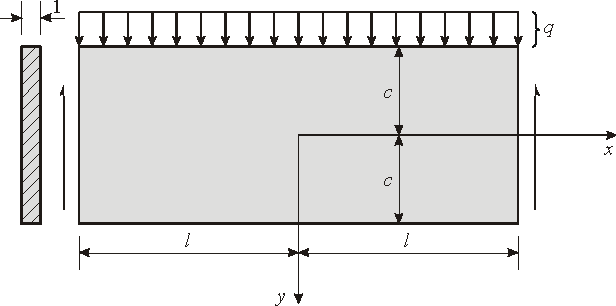
\includegraphics{ej6}
\end{center}

No hay fuerzas de cuerpo. Se sugiere que la distribución de tensiones sea

\begin{align*}
\sigma_{xx} &= \frac{q}{2I}(l^{2}-x^{2})y+\frac{q}{2I}\left(
\frac{2}{3}y^{3}-\frac{2}{5}c^{2}y\right) \\
\sigma_{yy} &= -\frac{q}{2I}\left(\frac{1}{3}y^{3}-c^{2}y+\frac{2}{3}c^{3}\right) \\
\sigma_{xy} &= -\frac{q}{2I}(c^{2}-y^{2})x \\
\sigma_{zz}=\sigma_{xz}=\sigma_{zy} &= 0 \\
\end{align*}

donde $q$ es la carga por unidad de área y $I=\frac{2c^{3}}{3}$ es una constante. Determine si la solución es correcta o no. 

\dotfill

\begin{align*}
\nabla\bullet\sigma &= 0 \\
\frac{\partial\sigma_{xx}}{\partial x}+\frac{\partial\sigma_{xy}}{\partial y} &= 0 
&& \implies & -\frac{2xyq}{2I}+\frac{2qxy}{2I} &= 0 \\
\frac{\partial\sigma_{yy}}{\partial y}+\frac{\partial\sigma_{xy}}{\partial x} &= 0 
&& \implies & -\frac{q}{2I}(y^{2}-c^{2})-\frac{q}{2I}(c^{2}-y^{2}) &= 0 \\
\sum F_{y} &= -F_{2}-F_{1}+F_{3}=0 \\
&= -F_{2}-F_{1}+2Lq=0 && \implies & F_{2}=-F_{1}+2Lq=-Lq+2Lq &= Lq \\
\sum M_{0} &= 2LF_{1}-L2Lq=0 && \implies & F_{1} &= Lq \\
\nu_{1} &= \begin{pmatrix}
0 \\
-1
\end{pmatrix} \\
t_{1}=\sigma\nu_{1} &= \begin{pmatrix}
0 \\
\frac{q}{2I}\left(-\frac{1}{3}c^{3}+c^{3}+\frac{2}{3}c^{3}\right)
\end{pmatrix}
=\begin{pmatrix}
0 \\
q
\end{pmatrix} \\
\nu_{2} &= \begin{pmatrix}
1 \\
0
\end{pmatrix} \\
t_{2}=\sigma\nu_{2} &= \begin{pmatrix}
\frac{q}{2I}\left(\frac{2}{3}y^{3}-\frac{2}{3}c^{2}y\right) \\
-\frac{q}{2I}\left(c^{2}-y^{2}\right)L
\end{pmatrix}
=\begin{pmatrix}
0 \\
-qL
\end{pmatrix} \\
\end{align*}

\section*{Apéndice}

\begin{enumerate}[1.]

\item \textit{Fluido no viscoso:}

\begin{align}
\sigma_{ij} &= -p\delta_{ij} & p=\rho RT
\end{align}

p: presión \\
$\rho$: densidad \\
R: constante de los gases \\
T: temperatura \\

Si el fluido es incompresible entonces la densidad es constante.

\item \textit{Fluido Newtoniano:}

\begin{align}
\sigma_{ij} &= -p\delta_{ij}+2\mu V_{ij}
\end{align}

\item \textit{Sólido elástico Hookeano:}

\begin{align}
\mbox{Ley de Hooke:} && \sigma_{ij} &= \lambda e_{\alpha\alpha}\delta_{ij}+2\mu e_{ij}
\end{align}

También se puede escribir como:

\begin{minipage}[t]{0.5\linewidth}

\begin{align*}
\sigma_{xx} &= \lambda(e_{xx}+e_{yy}+e_{zz})+2Ge_{xx} \\
\sigma_{yy} &= \lambda(e_{xx}+e_{yy}+e_{zz})+2Ge_{yy} \\
\sigma_{zz} &= \lambda(e_{xx}+e_{yy}+e_{zz})+2Ge_{xx} \\
\sigma_{xy} &= 2Ge_{xy} \\
\sigma_{yz} &= 2Ge_{yz} \\
\sigma_{zx} &= 2Ge_{zx} \\
\end{align*}

$\lambda$, $\mu$: \textit{constantes de Lamé}. \\

$E$: \textit{módulo de Young}. \\

$\nu$: coeficiente de Poisson. \\

$\mu=G$: módulo de corte. \\

\end{minipage} \hfill \begin{minipage}[t]{0.5\linewidth}

\begin{align*}
e_{xx} &= \frac{1}{E}(\sigma_{xx}-\nu(\sigma_{yy}+\sigma_{xx})) \\
e_{yy} &= \frac{1}{E}(\sigma_{yy}-\nu(\sigma_{xx}+\sigma_{zz})) \\
e_{zz} &= \frac{1}{E}(\sigma_{zz}-\nu(\sigma_{xx}+\sigma_{yy})) \\
e_{xy} &= \frac{1+\nu}{E}\sigma_{xy} \\
e_{yz} &= \frac{1+\nu}{E}\sigma_{yz} \\
e_{zx} &= \frac{1+\nu}{E}\sigma_{zx} \\
\mbox{Donde:} \\
\lambda &= \frac{E\nu}{(1+\nu)(1-2\nu)}           \\
G=\mu   &= \frac{E}{2(1+\nu)}                     \\
E       &= \frac{\mu(3\lambda+2\mu)}{\lambda+\mu} \\
\nu     &= \frac{\lambda}{2(\lambda+\mu)}         \\
\end{align*}

\end{minipage}

\end{enumerate}

\textit{Función de tensión de Airy:}

\begin{align*}
\nabla^{4}\Phi &= \frac{\partial^{4}\Phi}{\partial x^{4}}
+2\frac{\partial^{4}\Phi}{\partial x^{2} \partial y^{2}}
+\frac{\partial^{4}\Phi}{\partial y^{4}}=0
\end{align*}

\begin{thebibliography}{99}
\bibitem{MCF}
Y. C. Fung,
\emph{A First Course in Continuum Mechanics}, 
tercera edición,
PRENTICE HALL,
1994.
\end{thebibliography}

\end{document}